% !TeX spellcheck = en_US
\chapter{Background} \label{background}
\setcounter{chapter}{2}
\section{Colorectal Polyps, Medical Imaging, and Deep Learning}
	Polyps are small growths found in and around the inner lining of the large intestine. These polyps, also referred to as adenomas, can in time develop into cancerous tumours, or carcinomas, in a process known as the adenoma-carcinoma sequence \cite{ACS}. Though the majority of polyps do not undergo this process, identifying polyps nonetheless constitutes an important step towards preventing colorectal cancer. Indeed, resection of these polyps has been shown to reduce the incidence of colorectal cancer by a significant margin \cite{resection}. 
	
	Though colorectal cancer remains as one of the leading causes of cancer-related death worldwide (source), mortality rates have nonetheless declined in large part to increased use of screening colonoscopy, which in turn has facilitated the use of more preemptive treatment. Polyps are, however, by nature somewhat difficult to detect and are routinely missed by clinicians, with miss rates ranging upwards of 27\% for diminutive (<2.5mm) polyps  \cite{missrate1, missrate2}.
	
	Reducing this miss rate has the potential to further reduce incidence rates. As a result, there has been a significant body of work dedicated to developing systems and techniques to aid in optimizing and effectivizing the screening procedure. One such example, referred to as chromoendoscopy, has been shown to reduce miss rates by (...) merely by employing the use of specific dyes prior to the colonoscopy. Similarly, the use of narrow-band imaging techniques, wherein light of specific wavelengths specifically designed to highlight the textural differences between the polyps and the surrounding tissue, has been shown to reduce miss rates by (...) 
	
	These systems do, however, require more equipment, training and expertise to effectively employ. Thus, automatic polyp segmentation using deep learning and convolutional neural networks (CNNs) has been identified as a possible diminutive detection method. This requires minimal training time on the part of the clinician, no additional equipment, and has been show to significantly increase detection rates when deployed in a clinical setting \cite{polyp-success-story}. 

	This has spurred on a large body of research dedicated to improving on the performance and expanding the capabilities of deep-learning based systems for polyp detection and segmentation. Several challenges been also held, namely the Endotect challenge \cite{endotect}, EndoCV2020 \cite{endocv2020}, EndoCV2021 \cite{endocv2021}, and more.
	
	There are, however, still several hurdles to overcome; recent research has shown that even state of the art deep-learning pipelines are prone to generalization failure when deployed in practical settings, particularly when exposed to distributional shifts such as changes in demographics, imaging equipment, noise, and more despite exhibiting high performance on hold-out sets \cite{retinopathy, damour2020underspecification, pneumonia, shortcut_learning}. As a result, the EndoCV2021 challange emloyed training data from several centers, with the data from one of the centers being hidden and used as generalization test data. The results from this challange demomstrated the pervasiveness of generalization failure, with every submitted model exhibiting significant performance reductions when evaluated on their hidden dataset (cite summary here). 
	
	Naturally, automatic segmentation systems are rendered practically useless should they fail to perform sufficiently outside of the very carefully controlled conditions upon which they are trained. Consequently, for any such system to have any practical merit, it has to have the capacity to infer causally reasonable patterns in the data that generalize well to other hospitals, demographics, imaging equipment, resolutions, and so on. 

\section{Generalization failure in broader contexts} \label{case_studies}
	\subsection{Generalization failure in Medical Imaging}
	Generalization failure is not, of course, unique to the gastrointestinal domain. Indeed, though medical imaging has in recent years proven to be one of the most promising applications of artificial intelligence and deep learning, having the capacity to significantly improve both the accuracy and efficiency of detection, diagnosis, and treatment of a wide variety of diseases \cite{dl_medical_imaging}, they are nonetheless highly prone to generalization failure. In addition to the already limited capabilities of deep neural networks to generalise, medical domains are subject to a number of other exacerbating factors that make generalization all the more diffcult. Training data is often scarce, the pathologies that constitute the classification targets are unevenly distributed and often exhibit high degrees of within-class variability. Moreover, due to the sheer scope of the data involved, there are inevitably a significant number of confounding variables both during training and in deployment.  
		
	For instance, a deep-learning based classifier which successfully detected pneumonia in X-ray scans across a number of hospitals with striking accuracy was determined to be basing its predictions not on any lesions or otherwise pathologically relevant features in the images, but rather on a hospital-specific metal token that was on every image, which it used in conjunction with learning the prevalence rate of pneumonia for the hospitals from which the data was collected. As a result, when deployed on data from hospitals that it had not seen during training, the system failed to generalize \cite{pneumonia}. In another study, it was shown that a classifier intended to detect diabetic retinopathy exhibited significant variability in performance depending on the type of camera used. The same study also showed that the same type of performance variability could be found when detecting skin-conditions across demographics with differing skin tones. \cite{damour2020underspecification}. Finally, a model trained to detect and diagnose melanomas  was shown to in large part be basing its predictions on whether or not it could detect any pre-surgical markings, used by doctors to assist in surgery preparation, in the vinicity of the lesion\cite{skin_shortcut}.  
	 
	\subsection{Generalization failure in other domains}
	Naturally, non-medical domains are in no way immune to generalization failure. In fact, one could easily argue that the vast majority of deep-learning pipelines fail to generalize altogether, and instead merely infer some set of inductive biases that, although perhaps causally incorrect, perform sufficiently well for general use. It has for instance been shown that CNNs trained on imagenet, one of the largest and most diverse datasets in the domain of computer vision, are heavily biased towards textural features\cite{texturebias}. Naturally, this is not necessarily causally accurate; a cat is not a cat because it has cat-like fur; nor is an elephant an elephant only because it has skin of an elephant. By manually increasing shape bias, it has been shown that the performance of such CNNs improves both in robustness to perturbations and iid accuracy.

	\begin{figure}[h]
		\includegraphics[width=\linewidth]{example-image-a}
		\caption{}
		\label{cat_elephant}
	\end{figure}
	
	Another characteristic of deep learning that supports this argument is the effectiveness of adversarial attacks \cite{adversarial_bugs_features}, which specifically target weaknesses in the inductive biases within DNNs through any number of means in an attempt to induce high rates of incorrect, yet highly confident predictions. Gradient-based adversarial attacks, for instance, use the gradients of the model to break even the most sophisticated and well-trained pipelines merely by adding some carefully crafted, yet visually imperceptible noise to the inputs \cite{adversarial_attacks}. Even without access to the gradients, there exists a multitude of so-called black-box attacks that only use output samples to generate similarly effective attacks (cite). Finally, it has been shown that adding minor visual distractions to objects, for example adding bits of tape or graffiti to stop signs, dramatically increases misclassification rates \cite{physical_attacks}. 
	
	Even benign, but nonetheless confounding perturbations also have the potential to induce failure. It has for instance been shown that sophisticated natural language processing models can and readily do fail if one adds peripheral information to the input. (Example, citation)	 
	
\section{Generalisability Theory}
	Exactly why and how DNNs seem to so persistently fail to generalize is a topic of ongoing research, and the available literature seems to suggest that the problem is multifaceted. This section is an attempt to summarize and distill the findings and analysis performed in the field. It will cover the theoretical basis of generalization and why one might expect DNNs to generalize, discuss the key characteristics of generalization failure and their origins, and finally introduce a probabilistic perspective of generalization.
	\subsection{Generalization through Empirical Risk Minimization} 
		Naturally, deep learning would not have experienced as much of a revolution in the last decade or so if there was not some semblance of an expectation that their striking performance was generalisable and performant also outside the idealized settings typically involved in research. The theoretical basis that informs this belief in (most) modern deep learning pipelines is the idea of so-called empirical risk minimization, wherein it is assumed that the dataset upon which the model is trained is a representative sample of the distribution of all possible samples in the relevant domain. In other words, it assumes that the dataset is independently and identically distributed (iid) to the domain distribution. To better understand this assumption, it is beneficial to consider the it from first principles: 
		
		At the most fundamental level, the goal of machine learning is to learn a mapping between two spaces of objects \(X\) and \(Y\). This mapping, namely the function \(f: X \rightarrow Y\), maps some input object \(x \in X\), an image for example, to a corresponding and application-relevant output object \(y \in Y\), for instance a segmentation mask or a class probabilities. It is worth noting, however, that \(f\) is not as much a function in the mathematical sense as much as it is an abstraction of whatever ground-truth relationship that the deep learning system is intended to capture, and consequently cannot typically be modelled explicitly. Instead, machine learning systems aim to find a representation of this mapping automatically by leveraging a training set \(\{x_i, y_i\}_{0...n}\) to find a sufficiently performant approximation of \(f\). This is referred to as supervised learning, and the resulting approximation found using the training set is denoted by \(h: X \rightarrow \hat{Y}\), and typically referred to as a hypothesis.  
		        
		To find such an approximation, we assume that there exists a joint probability distribution over \(X\) and \(Y\), namely \(P(x,y)\), and that the training data \(\{x_i, y_i\}_{0...n}\) is drawn from this probability distribution such that the resulting sample distribution is independent and identically distributed to \(P(x,y)\). This is the so-called iid assumption. By modelling the mapping as a joint probability distribution, one can model uncertainty in the predictions by expressing the output as a conditional probability \(P(y|x)\). In conjunction with a loss-function \(L(h(x),y)\) which measures the discrepancy between the hypothesis and the ground truth, these assumptions allows us to quantify the expected performance of a given hypothesis:
		\begin{equation}
		    R(h) = \boldsymbol{E}[L(h(x),y)] = \int L(h(x),y) dP(x,y)
		\end{equation}
		Using this framework, one can then find an iid-optimal hypothesis, often called a predictor, by finding the predictor \(h^*\) among a fixed class of functions (defined by network architecture) \(\mathcal{H}\) that minimizes risk:
		\begin{equation}
		h^* = \argmin_{h \in \mathcal{H}}R(h)
		\end{equation}
		
		Since \(P(x,y\)) is not known, however, one cannot compute \(R(h)\) explicitly. Instead, the expected risk has to be estimated empirically, i.e by finding the arithmetic average of the risk associated with each prediction by the hypothesis over the training set:
		\begin{equation}
		R_{emp}(h) = \frac{1}{n}\sum_{i=1}^{n}L(h(x_i), y_i)
		\end{equation}
		This risk can in turn be minimized with respect to the hypothesis class. This is called empirical risk minimization (ERM):
		\begin{equation}
		\hat{h} = \argmin_{h \in \mathcal{H}}R_{emp}(h)
		\end{equation}
		To reiterate, the central idea with this approach to machine learning is that the training data can be considered a finite iid sampling of the underlying distribution. As such, by the central limit theorem, the hold-out performance of the computed hypothesis will approach iid-optimal performance given a sufficient amount of training data and some sufficiently capable and regularized training procedure. This should in theory allow deep learning systems to be able to generalize, since the empirical risk in theory can approximate the true risk arbitrarily well given sufficient training data support.
	\subsection{Understanding Generalisation}
		As the analysis in \ref{case_studies} shows, ERM nonetheless readily fails to generate generalizable predictors with respect to out-of-distribution data). Understanding exactly why this is the case is a subject of ongoing study, and cannot be uniquely attributed to any one property of the machine learning pipeline. In broad strokes, the literature attributes generalization failure to two key properties of modern deep learning pipeline, namely that DNNs readily learn non-robust features, and that DNNs are underspecified by the training data. 
		Naturally, there is some degree of overlap between these two views, and both phenomena induce similar behaviour. In an attempt to systematize the To fully understand the nuances that distinguish the respective arguments, it is useful to first consider the assumptions upon which ERM is based, namely that: TODO: FIX
		\begin{enumerate}
			\item \(f\) exists in \(\mathcal{H}\) \label{underfit}
			\item \(R_{emp}\) is sufficiently sampled \label{overfit} %todo refactor
			\item \(\{x_i, y_i\}\) is an IID sampling of \(P(x,y)\). This is the aforementioned iid assumption. \label{structural_misalignment}
			\item \(\hat{h}\) is unique in \(\mathcal{H}\)\label{underspecification}
			\item The optimizer consistently finds \(\hat{h}\) (given that it exists and is unique)\label{opt}
		\end{enumerate}
		As the following sections will show, violations of any one of these assumptions can and typically will result in generalization failure.  

	\subsection{Underfitting, Overfitting and Regularization}
		Violations of assumptions \ref{underfit} and \ref{overfit} correspond to well known and fairly well understood forms of generalization failure, namely underfitting and overfitting. One can however argue that these factors can be all but discounted as plausible explanations for the pervasiveness of generalization failure. 
		
		Underfitting occurs when the model simply lacks the complexity required to encapsulate the patterns necessary to form generalizable predictions. To give a simple example - consider the problem of trying to fit a linear model to the following dataset: 
		\begin{figure}[h]
			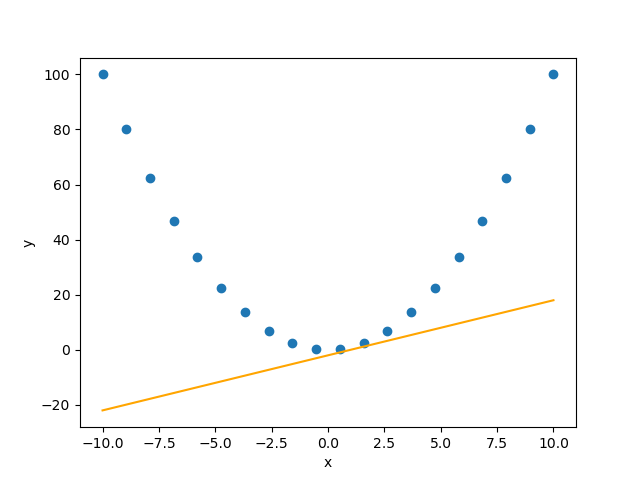
\includegraphics[width=\linewidth]{illustrations/regression_example.png}
			\caption{A linear model cannot fit polynomial data}
			\label{underfit example}
		\end{figure}
		Obviously, no amount of optimization of the parameters in the linear model can ever result in a sufficient description of the underlying data and the function it follows, namely \(y=x^2\). 
		
		It is commonly accepted that DNNs are not particularly susceptible to underfitting. Modern DNNs, as it turns out, can after all be shown to have infinite effective capacity for practical purposes. It can for instance be shown that even a 2-layer feedforward neural network is capable of fitting noise to random labels with 100\% accuracy \cite{randomlabels}. Assuming this ability translates to a capacity to generalize (which may not necessarily be the case, as will be discussed in chapter \ref{discussion}), it is fairly reasonable to expect that the hypothesis space of the highly complex models used today contains a generalizable predictor. 

		This is also evidenced by the fact that practically all deep learning pipelines take considerable steps towards avoiding the exact opposite of underfitting - overfitting. Overfitting occurs when the model learns patterns that by conventional wisdom are too complex to be likely to actually describe the process(es) that generate them. Once again, to give a somewhat simple example: 
		\begin{figure}[h]
			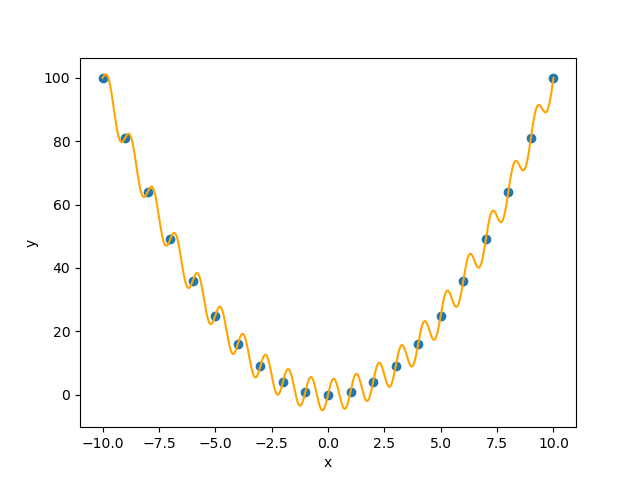
\includegraphics[width=\linewidth]{illustrations/overfit.png}
			\caption{A model with excessive capacity interpolates unneccesarily complex patterns}
			\label{Overfit example}
		\end{figure}
		The underlying function is once again \(y=x^2\). The sinusoidal pattern in the interpolated function is obviously erroneous, but this is impossible to determine with complete certainty given only a finite sampling of the underlying function. More generally, every finite sampling of any function can be interpolated as any one of an uncountably infinite set of functions. To prove this, consider the task of finding a function that fits the series \((1,4,9)\). Though ones first instinct would be to assume the pattern is described by the function \(y=x^2\), and that the next number in the sequence thus is 16, the next number can really be anything at all. Using Newton interpolation, or for that matter any arbitrary interpolation scheme, one can easily find a polynomial that fits the sequence \((1,4,9,n, n \in \mathbb{R}\). Since the set of real numbers is uncountably infinite, it follows that the space of functions that fits this new sequence also is uncountably infinite, depending on \(n\). Thus, there is an uncountably infinite number of functions that describe \(1,4,9\) as well. This of course does not only apply to extrapolating the next element in a sequence, but also any interpolating between consecutive elements. TODO clarify
		Naturally, this also applies to neural networks. Though instead of discrete sequences, it is probability distributions that are being modelled. Just like how extrapolation and interpolation between points is ill-defined for sequences, it is ill-defined for probability distributions. Consequently, it is necessary to introduce a number of assumptions and constraints to the problem. (CLARIFY)
		
		Obviously, the minimum level of generalization one should achieve is generalization to iid data. To this end, it is necessary to incorporate an iid evaluation method, such as keeping hold-out sets, cross validation, etc. This is of course ubiquitous in modern deep learning. Moreover, it is necessary to make some assumptions regarding the simplicity - or rather, complexity - of the resulting predictor. Certain neurons should for instance not dominate the predictions, the weights should have reasonable values, etc. This is what motivates so-called regularization, whereby different methods - for instance batch normalization, drop-out, L2 loss, weight decay, etc - are used to bias the search towards areas in the loss landscape that are more credible from a perspective of model complexity. This is of course only necessary because assumptions \ref{overfit} and \ref{underspecification} do not hold. Given a perfect (or at least very well sampled) representation of the risk and consequently the loss-landscape and a perfect optimizer, the model would not overfit in any meaningful way.  

		Regularization has of course for this reason been extensively studied, and for most purposes the existing regularization techniques suffice just fine for IID data, and typically yield highly performant predictors so long as it is not subjected to any form of distributional shift. Consequently, Overfitting, though naturally still a factor that needs to be accounted for when designing deep learning pipelines, is not at fault for the generalization failure that is exhibited in modern deep learning systems.

		%Connective paragraph here

	\subsection{Structural Misalignment and dataset bias}
		Generalization failure is often attributed to structural misalignment between the predictor as generated by ERM and the causal structure which it ideally should encode \cite{adversarial_bugs_features,shortcut_learning,IRM, causality}. Generally, this misalignment occurs as a result of the predictor learning spurious or otherwise causally unrepresentative features that nonetheless perform well within the training distribution. This if of course made evident as soon as the predictor is exposed to any form of distributional shift, at which point it will (typically) fail to generalize. These distributional shifts can range in magnitude, from changes in imaging modalities, common corruptions such as noise or blurs \cite{benchmarking_robustness} or spatial transforms \cite{spatial_robustness} to practically imperceptible perturbations, typically exemplified by adversarial attacks \cite{adversarial_attacks}. ERM does not and cannot guarantee invariance to distributional shifts, as it assumes that the training data is IID to \(R(h)\). This is not, however, necessarily as much of a flaw with ERM inasmuch as it is a flaw in the reasoning behind our expectations. 
		
		To illustrate, consider the rather pertinent example of training a model exclusively on either white-light or narrow-band endoscopy. Assume that there are two datasets, each containing samples depicting identical scenes, with the only difference being that dataset A employs white-light endoscopy, whereas dataset B employs narrow-band endoscopy. Ideally, a model trained on either dataset should generate predictors that can generalize to the other, and though one may be optimistic and hope this is the case, this is in no way guaranteed. The causal structure behind the decisions - i.e what exactly makes a polyp a polyp - is never considered at any point in the training process. Instead, the models will simply try to leverage whatever predictive patterns can be found the training data. The model trained on narrow-band images may for instance principally consider the textural characteristic of the polyps, which narrow-band endoscopy enhances. Conversely, the model trained on white-light, lacking access to these textural characteristics, may instead consider more color- or shape-based features. Naturally, if this narrow-band-texture-biased model is deployed in white-light endoscopy, it is not likely to succeed since its principal discriminative features no longer are particularly useful. Similarly, the color-biased model would fail when deployed in narrow-band endoscopy since the colours it once used to distinguish polyps are no longer predictive in narrow-band images.  

		\begin{figure}[h]
			\includegraphics[width=\linewidth]{example-image-b}
			\caption{}
			\label{imaging_modalities}
		\end{figure}

		Though the features each model learns are not particularly representative of the broader context of what makes a polyp a polyp, they make sense when considered from the perspective of either of the two hypothetical modalities. When considering only narrow-band imaging, it makes some sense to heavily weigh the texture of the polyps. When considering only white-light imaging, it makes some sense to heavily weight the shape and colour of the polyps. Though humans are capable of appreciating broader context and subconsciously know that certain features are ancilliary rather than causal (and perhaps more importantly: know the strengths and weaknesses of each modality), DNNs lack the inductive biases needed to take this into account. Once again, DNNs merely leverage the first and best predictive patterns found during the training process, and cannot be expected to optimize for specific invariances on their own, irrespective of how self-evident these invariances may be for humans. This predilection towards dataset-specific features is aptly referred to as dataset bias. 
		
		\subsubsection{Shortcut Learning}
		In the aforementioned example, tough the features each predictor learns is not robust to dataset shift, they nevertheless have causal explanations. The causal structure that they correspond to is of course not dataset-agnostic, and as a result flawed in their own way, but the patterns the respective models leverage to interpret the data are not particularly irrational. As it turns out, however, DNNs are unlikely to learn such causally viable features in the first place. In other words, the predictors would not necessarily learn to consider texture in narrow-band images - it could learn any arbitrary pattern so long as it is predictive. Moreover, if such interpretable distributional shifts were the principal cause of generalization failure, generalizability could be induced by explicitly modelling the effects such shifts induce and taking this into account in the pipeline. In the aforementioned example, one could for instance train some model to map from one lighting environment to the other. Though this would imbue the model with an inherent invariance to the choice of lighting, it is nonetheless not given that the resulting model will be perfectly generalizable.

		Consequently, though these detectable forms of distributional shifts also hold some importance when designing generalizable models, a more pervasive and substantially more significant issue is the fact that many of the distributional shifts encountered in clinical settings are not necessarily considered significant or for that matter at all perceptible to a human observer. A human would for instance not be significantly affected by slightly noisy, blurry, rotated, or compressed images, nor would they in all likelihood notice these perturbations. DNNs, on the other hand, have been shown to be highly sensitive to these and several other forms of minor perturbations \cite{noise_robustness, corruption_robustness,adversarial_training,benchmarking_robustness}. Moreover, a human would likely not pick up on the subtle phenotypic cues that may exist in the colon during endoscopy, whereas a DNN may leverage some of these cues to inform their decisions. 

		It is important to note, however, that despite how these two forms of distributional shift may at surface level appear as completely seperate classes of problems, they can both be traced to the same phenomena - namely that DNNs do not leverage any form of causal logic to inform their decisions and, as mentioned previously, simply exploit any sufficiently predictive pattern they may observe in the data. This phenomenon has been shown to be pervasive across all manner of domains, from natural language processing and computer vision to reinforcement learning and algorithmic decision making. This is referred to as shortcut learning \cite{shortcut_learning} or the Clever Hans effect \cite{cleverhans}. 
		%Connection to shortcut learning
		Shortcut learning and the brittle features it corresponds to have also been identified as one of the key properties that explains the effectiveness and pervasiveness of adversarial attacks \cite{adversarial_bugs_features}. Naturally, a generalizable predictor should be robust to such minor perturbations, as the model should not in the first place be learning features that get perturbed to any significant degree by adding such high-frequency, low-amplitude noise. Adversarial attacks simply leverage the high degrees of sensitivity inherent to shortcut features, and construct perturbations according the direction in the search space that corresponds to the principal component of this sensitivity \cite{sensitivity}. 


	\subsection{Underspecification}
		Closely related to shortcut learning is underspecification \cite{damour2020underspecification}. A machine learning pipeline can be considered underspecified when it can return any number of risk-equivalent predictors when evaluated on an iid holdout set, dependent only on the random variables used within the training procedure - i.e dropout, seed initialization, and so on. Even with identical hyperparameters, a given training procedure can return any number of predictors each having learned different patterns. One predictor may have learned one shortcut, another may have learned a different shortcut, and one may have fully learned the actual causal relationships it is intended to. With ERM, and in particular with iid-oriented evaluation procedures, these are all erroneously considered equivalent. 

		Note that this does not however presuppose anything about the relative occurrence rates of generalizable and non-generalizable predictors. It may not necessarily even be the case that the pipeline can return a generalizable predictor at all. Only that there exists a multitude of risk-equivalent predictors in the search space the optimizer typically explores. Nor does it presuppose anything about the distribution of predictors, only that there is indeed a distribution. 

		This is evidenced by the fact that generalizability can vary greatly depending on the choice of random seed used during training. In the foundational paper on underspecification in deep learning, for instance, it was highligted that certain classification pipelines can produce predictors that vary in ood accuracy by up to 10\% \cite{damour2020underspecification}. This is a function of the robustness of the learned features and how likely the pipeline is to return the corresponding predictors. 
	\subsection{A probablisitic perspective of generalization}
		As established, modern deep learning pipelines are not capable of reliably returning generalizable predictors. However, they are not necessarily precluded from it. One can to some extent model this probabilistically by considering the distribution of parameters given the training data, \(p(w | \mathcal{D})\). Though it is impossible to know which part of this distribution corresponds to generalizable predictors, it has been shown that marginalizing over this distribution - in other words, bayesian learning - increases generalizability \cite{bayesian_generalization,endoensemble,divergentnets,ensemble_machinereading}. 

		\cite{bayesian_generalization} provides a probabilistic perspective of this phenomenon. They consider generalizability as a two-dimensional quantity, consisting of the support and inductive biases of a model.

		\section{Related work on generalizable deep learning}
	To summarize, generalization failure occurs due to the weaknesses inherent to ERM. The features that ERM learn to incorporate are often spurious, and the predictors that leverage them are often returned practically arbitrarily from the pipeline. The approaches that have exhibited the highest degrees of success towards increasing generalization as a consequence tend to address these issues in some way or another. 
	
	One of the most well-studied approaches to increasing generalizability is the use of data augmentation. Data augmentation is typically implemented in deep learning pipelines in order to prevent overfitting, often in conjunction with other regularization methods. Naturally, overfitting also constitutes generalizability failure in its own right, but augmentation has also been shown to have positive effects for out-of-distribution generalization. It has for instance been shown that carefully designing augmentation procedures increases the generalizability of polyp segmentation models \cite{polyp_augmentation} and prostate segmentation \cite{augmentation_prostate}. There has also been a large body of work dedicated to leveraging recent advances in generative models such as generative adversarial networks (GANs) and variational autoencoders (VaEs) to serve as synthetic data augmentation. These types of approaches have also been been shown to increase generalizability in CT segmentation \cite{cyclegan} and x-ray based covid detection \cite{covid}. Data augmentation facilitates generalization by implicitly biasing the pipeline towards credible inductive biases, as the empirical risk will be best minimized by leveraging features that are conducive to minimizing risk across both synthetic or otherwise augmented data and unaugmented data. Naturally, the choice of augmentations that are used is an inductive bias in and of itself; by employing random rotations, rotational invariance is presupposed. By employing random cropping, image-space object size invariance is presupposed. By employing additive noise, invariance to additive noise is presupposed, and so on. From an ERM perspective, this corresponds to improving the empirical risk estimate; given enough data, all of these invariances may be learned automatically. With a finite and often fairly limited dataset, this may not necessarily be the case simply due to the large number of confounding variables involved. 

	Another type of approach involves biasing the pipeline towards learning more structured and causally viable latent representations. This is also somewhat well understood when considered through the lens of regularization: drop-out and weight-decay are often employed in order to reduce overfitting under the assumption that a generalizable predictor should not base its decisions on only a few of the available neurons and that seperate neurons should instead encode independent representations of the input. Though there is limited research ont the effects of dropout on ood generalization, constraining the latent representations in DNNs has been shown to be effective method to increase generalizability. For polyp-segmentation it has for instance been shown that adding context-based attention layers to multiple blocks in a given network results in state-of-the-art IoU scores for out-of-distribution evaluation on certain datasets \cite{uacanet}. Other attention-based approaches have also shown promise in this regard \cite{attention_generalizability, reverse_attention}. This permits the model to learn and generate attention maps for its latent representations, thus in theory biasing the model towards learning more a more structured interretation of the data. 
	
	Multi-task and/or multistage learning has also been leveraged to this end. By jointly optimizing for multiple tasks/subtasks, the model can be biased towards learning features that describe the input data well independent of their performance on any one of the relevant tasks. For poylp-segmentation, for instance, it has been shown that adding image reconstruction as an auxiliary task \cite{ddanet} or decoupling the segmentation task into a coarse segmentation and refinement stage \cite{doubleencdec} increases generalizability. 

	More closely supervised methods, wherein certain inductive biases have been explicitly introduced to the pipeline, have also been shown to have some promise. One paper for instance reported an increased robustness to image perturbations after adding a custom filter bank designed to emulate the primary visual cortex of primates to the front of the CNN \cite{visual_cortex}. Another reported that models trained on imagenet exhibited significantly higher robustness when explicitly biased towards shape-based features \cite{texturebias}. 
	
		
	These approaches all provide workarounds to flaws with ERM, typically to limited practical effect. Consequently, a growing body of work has instead been investigating the idea of foregoing ERM altogether in favor of developing alternative training paradigms. In so-called Invariant Risk Minimization\cite{IRM}, for instance, the model trains to ignore spurious correlations by optimizing for predictors that exhibit stable performance across multiple training environments. A similar approach, namely model-based robust deep learning \cite{modelbased}, employs a similar idea in conjunction with distributional modelling. The model is trained such that it is robust to perturbations as generated by a so-called model of natural variation. If this model for instance describes the function mapping one training environment to another, this will then optimize for predictors that are invariant to the distributional shift this function corresponds to. 

	Finally, Bayesian learning has also been shown to improve generalization. In particular, ensemble-based networks - which mathematically can be considered an approximation of Bayesian marginalization \cite{bayesian_case,bayesian_generalization} - have demonstrated high degrees of generalizability for polyp-segmentation \cite{divergentnets,endoensemble}. Since deep learning pipelines are typically underspecified, one can consider an ensemble of predictors to be a sampling of the distribution over parameters given training data. These predictors are of course unlikely to have learned identical representations, and consequently whatever spurious correlations inferred by one predictor may be countered by the features employed in another. Consequently, features that are stable across predictors and consequently more likely to generalize are weighed to a greater extent, in turn mitigating the effects of underspecification. Structural misalignment may nevertheless impact ensembles, and as such the effective returns are limited. 

\section{Putting it all together}
	To summarize, generalizability failure can in broad strokes be attributed to the fact that ERM does not and cannot differentiate between causal and non-causal patterns, and that there typically exists multiple equivalent predictors in the parameter space of any given DNN model. Consequently, increasing generalizability boils down to the following questions:
	\begin{enumerate}
		\item How can behaviour consistent with the causal structure of a problem be rewarded? \label{loss}
		\item How can the inductive biases that underpin this causal structure be expressed? \label{mnv}
		\item How can we optimize for causally consistent inductive biases?\label{training}
	\end{enumerate}
	